\documentclass[../main.tex]{subfiles}

\begin{document}

\chapter{The Analytical Method}
\label{dts:chapter:intro}


The `Analytical Method' (AM) \textcolor{red}{[reference to AM paper]} is an algorithm developed for performing muon trigger primitive (TP) generation for Phase-2 in the CMS barrel by using information from the DT systems. It profits from the improved time digitization in Phase-2 DT input hits, 25/32 ns ($\equiv1$~TDC count), much finer than the 25 ns needed for bunch crossing (BX) identification. The muon segment parameters (position and direction) will have a resolution comparable to what is reachable with the present offline reconstruction software \cite{intro:id:muon_7tev}.



\section{Description of the algorithm}
\label{sec:dts:description}

This section describes the algorithm as included in both the software emulator and the firmware implementation. The algorithm can be logically separated in different parts, as shown in Fig.~\ref{dts:fig:am}. The inputs to it are only the time and cell number of all signals collected in each SL. In the first part of the algorithm, both $\phi$ SLs are treated independently, starting by combining the available hits into groups and then fitting into SL TPs. Finally, a correlation between the TPs coming from both SLs is attempted. 

Each logical step is further explained below.





\begin{figure}[h!]
\begin{center}
\includegraphics[width=0.6\textwidth]{Images/AM.pdf}
\end{center}
\caption{Sketch of the structure followed by the AM algorithm. The same four steps independently are followed for each $\phi$ SL, before a correlation between SLs is attempted.}
\label{dts:fig:am}
\end{figure}


\subsubsection*{Grouping}

In this step, the aim is to build \textit{cell layouts}, patterns of three or four signals in a given superlayer whose cells are compatible with a muon crossing the chamber in a straight trajectory, i.e. the ones shown in Fig.~\ref{dts:fig:cell_layouts}. These patterns are built synchronously whenever a hit is detected and introduced as input to the algorithm.

\begin{figure}[h!]
\begin{center}
\includegraphics[width=\textwidth]{Images/cell_layouts.pdf}
\end{center}
\caption{Sketch of the cell layouts compatible with straight muon trajectories in a DT chamber.}
\label{dts:fig:cell_layouts}
\end{figure}

Whenever a new hit is detected and introduced as input to the algorithm, it is stored and compared with all the hits that were previously stored and that could be used to build one of the eight available cell layouts. These is done by looking at ten cells at once, shown in Fig.~\ref{dts:fig:triangle}, which would depend on the layer of the new hit. Then, a loop is performed to build the cell layouts of Fig.~\ref{dts:fig:cell_layouts} from left to right. Each cell layout will be considered only if at least one hit in at least three of the four associated cells are available. If more than one hit per layer is available, all the possible combinations are built.

\begin{figure}[h!]
\begin{center}
\subfloat{\includegraphics[width=0.45\textwidth]{Images/pivot0.pdf}}
\subfloat{\includegraphics[width=0.45\textwidth]{Images/pivot1.pdf}}\\
\subfloat{\includegraphics[width=0.45\textwidth]{Images/pivot2.pdf}}
\subfloat{\includegraphics[width=0.45\textwidth]{Images/pivot3.pdf}}
\end{center}
\caption{Structures of 10 cells where the combinations of three or four hits are looked for. The cell shown in red indicates the one that detected the hit under study. Blue arrow indicates the first combination of cells that is studied, while the green one the last one.}
\label{dts:fig:triangle}
\end{figure}

\subsubsection*{Laterality prediction}

As was shown in Section~\ref{intro:sec:subdet_muon}, there is a left-right (laterality) ambiguity problem on the hit position. This step in the algorithm aims to provide all posible laterality combinations feasible for each cell layout. 

Due to geometrical constraints, at most four laterality combinations are available per cell layout. However, this number can be reduced by also considering the timing information from each hit in the group. The strategy to follow is, instead of considering the full timing information (which will be done later in the fitting), obtain for each hit the time difference with respect to the one in the group with the highest time value. These time differences are then compared to some thresholds to produce a set of three of four values from zero to three (\textit{coarsed set}) in a process called \textit{coarsification}. The combination of the set obtained and the cell layout are associated via a previous classification to up to three laterality combinations. 

To obtain the thresholds needed for the comparison and the laterality combinations available for each cell layout and coarsed set, a dataset of straight tracks (simulating a muon crossing a DT superlayer) is produced. These tracks follow the equation
\begin{equation}
x = x_0 + \text{slope} \cdot y,
\end{equation}
where $x$ is the position in the horizontal axis and $y$ the position in the vertical axis. $x_0$ and slope are given values between -21~mm and 21~mm and between -1.6 and 1.6 respectively (with granularities of 0.2~mm and 0.005). Each track gives a total of four hits, one for each layer, and from the position of each hit inside the cell both the drift time and the laterality can be extracted. To account for the detector resolution, each drift time is smeared by adding a random quantity sampled from a normal distribution with zero mean and $\sigma$ = 10~ns. 

Once the dataset is built, a dedicated algorithm is used in order to find the optimal thresholds for the coarsification. The algorithm tries to minimize number of coarsed sets for each cell layout that are associated to four or more laterality combinations by applying Bayesian optimization techniques \cite{dts:bayes, dts:bayes_python}. Two sets of thresholds are then selected, one for four-hit primitives and another one for three-hit primitives. With these sets of thresholds, 99.98\% (100\%) of the four-(three-) hit primitives in the training dataset will be selected if at most three laterality combinations are associated to each coarsed set.


\subsubsection*{Fitting}

After building the hit patterns and for each laterality combination obtained in the previous step, the muon primitive's time $t_0$, the bunch crossing (BX) of the proton-proton interaction that produced the muon, the segment local position and local direction with respect to the chamber perpendicular axis $\tan\psi$ are computed in a given superlayer using formulas extracted using the least squares minimization method. The $\chi^2$ of the fit is also computed.

%Among all the 4-hit candidates, only the hit laterality combination resulting in the smallest value for the fitted $\chi^2$ is selected. However, for groups of 3 hits all hit laterality asumptions that provide physical solutions are considered as candidates.

\subsubsection*{Confirmation}

Previous to the correlation between SLs, another step aimed to select the best single-SL TPs is performed. Each TP is \textit{confirmed} if, after extrapolating it to the other SL, this extrapolation matches to at least two hits. If this is the case, the segment gets tagged as a \textit{confirmed} segment candidate.

Once this confirmation is done, a quality code is assigned to each SL TP, as shown in Table~\ref{dts:tab:quality_sl}. By comparing this quality code between TPs, a filtering is done as follows:

\begin{itemize}
\item If two primitives have at least one hit in common, only the primitive with the highest quality is kept. In this way, a confirmed 4-hit TP prevails over a non-confirmed 4-hit, which prevails over confirmed and non-confirmed 3-hit TPs.
\item If two equal-quality TPs have at least one hit in common, the behaviour depends on the quality considered. For both 4-hit and 4+2 hits TPs, the TPs with the smallest $\chi^2$ obtained in the fitting prevails. For 3-hit and 3+2 hits TPs, as the $\chi^2$ is meaningless, both TPs are kept.
\item If no hit is shared between two TPs, both are kept, regardless of the quality of each of them.
\end{itemize}

\begin{table}[h!]
	\centering
	\begin{tabular}{c|c|c}
		Quality & Description & Type \\\hline
		1 & 3-hit TP & Uncorrelated \\
		2 & 3+2 hits TP & Confirmed \\
		3 & 4-hit TP & Uncorrelated \\
		4 & 4+2 hits TP & Confirmed
	\end{tabular}
	\caption{SL quality descriptions.}
	\label{dts:tab:quality_sl}
\end{table}


\subsubsection*{Correlation}

If at least one fit was obtained in each of the two $r$-$\phi$ SLs, a combination of those fits can be performed if their corresponding times lay in a window of $\pm 25$ ns. In that case, a fitting is performed again using the up to eight hits used in the SL-fits, obtaining new values for the $t_0$, BX, local position and local direction. The corresponding SL input segments are then discarded. If no match is found, all SL candidates are then kept at this stage. 

Depending on the number of hits used for the correlation, the quality code is updated with the new numbers described in Table~\ref{dts:tab:quality_cor}.


\begin{table}[h!]
	\centering
	\begin{tabular}{c|c|c}
		Quality & Description & Type \\\hline
		6 & 3+3 hits TP & Correlated \\
		7 & 4+3 hits TP & Correlated \\
		8 & 4+4 hits TP & Correlated
	\end{tabular}
	\caption{Quality descriptions.}
	\label{dts:tab:quality_cor}
\end{table}

A final filter is performed at this stage similarly to the SL-filter:
\begin{itemize}
\item If two TPs match (within given position, local direction and time ranges) and they have different quality, only the one with the highest quality remains. If they have the same quality, the one with the smallest re-fitted $\chi^2$ is kept.
\item If they do not match, both TPs prevail.
\end{itemize}


\section{Algorithm performance}
\label{dts:sec:performance}

In order to estimate the AM performance, several sets of simulated and real data samples have been used. For the results presented in this chapter, we will consider a 3700 simulated event sample with four prompt muon pairs per event. Each pair consists of 2 back-to-back generated muons with flat $p_T$, $\phi$  and $\eta$ distributions with a $p_T$ between 2 and 200 GeV and within $|\eta|<1.2$. Overimposed to the signal, additional proton-proton interactions (PU) are generated within a window of $\pm16$ BX around the central BX (where the signal muons are generated), fully covering the maximum drift time of $\sim$390~ns, with an average PU of 200 events per bunch crossing. Additionally, the GEANT4 \cite{geant} simulation configuration takes into account backgrounds from long-lived particles originating from collisions, in particular low-energy neutrons, that can produce hits in the DT chambers evenly over the LHC orbit. The simulation assumes a perfect inter-chamber calibration.

During Phase-2, DT chambers will be exposed to high radiation levels, specially in some regions of the detector, potentially producing aging effects degrading the DT cell performance and lowering the DT chamber efficiency. Several DT ageing scenarios can be simulated by removing in a random way DT hits, according to predefined probabilities. In our results, a scenario equivalent to 3000 fb${}^{-1}$ has been considered, corresponding to extreme ageing effects in the DT detector at the end of Phase-2. This conservative scenario has been based on measurements of the DT chamber performance under high radiation conducted in the new CERN Gamma Irradiation Facility. Theses hit efficiencies have been estimating considering a safety factor of 2 from the expected HL-LHC instantaneous luminosity (2$\times 5\times 10^{34}$ cm${}^{-2}$s${}^{-1}$) and the same safety factor for the expected integrated luminosity ($2\times$3000 fb${}^{-1}$). In this scenario, the lowest DT chamber efficiencies are in the order of 70$\%$ in MB1 of the most external barrel wheels (Wh $\pm2$), raising to 90$\%$ in some sectors from the MB4 and remaining significantly higher for the rest of the DT chambers, as can be seen in Fig.~\ref{dts:fig:ageing}. Despite these values, thanks to the redundancy of the system and to the mitigation measures currently implemented, a good performance of the muon triggering and reconstruction in still expected during Phase-2.

\begin{figure}[h!]
\begin{center}
\includegraphics[width=0.5\textwidth]{Images/EfficienciesAging_3000fb_v2}
\end{center}
\caption{Expected hit efficiencies at the end of Phase-2 for all the DT chambers of the CMS muon system. The upper plot shows MB4 chambers, the lower shows MB1, MB2 and MB3.}
\label{dts:fig:ageing}
\end{figure}

\subsection{Efficiencies to trigger on prompt muons}

In order to obtain TP efficiencies, the denominator is obtained as the number of DT offline segments with at least 4 hits in the r-$\phi$ view and also 4 hits in the r-z view (if available) geometrically matched with a generated muon within a window of 0.15 in $\eta$ and 0.1 rad in $\phi$. In order to remove segments coming from PU events, a cut on the reconstructed segment time of $\pm 15$ ns is applied. The numerator of the efficiency is defined as the number of trigger primitives whose BX is the one from the collision and matching these segments within a $\phi$ window of 0.1 rad.

Fig.~\ref{dts:fig:efficiency} summarizes the DT Phase-2 TP efficiency per station and wheel for two ageing scenarios: with no ageing applied and with the ageing scenario corresponding to 3000 fb${}^{-1}$. In both cases, 4 different TP quality thresholds are considered. When no ageing is considered, TP efficiencies are higher than 98$\%$ for a quality threshold of 1 or 2, while the efficiency for correlated TPs is above 80$\%$ in the whole detector. When the 3000 fb${}^{-1}$ ageing scenario is applied, the efficiency drop is larger in the chambers more affected by these ageing effects (as expected), overall for high TP quality thresholds. When lower qualities are considered, the efficiency can be substantially recovered.


\begin{figure}[h!]

\begin{center}
\subfloat[]{\includegraphics[width=0.45\textwidth]{Images/hEff_AM_rossin_noRPC_withAgeing_ext_confok_alignTrue_0}}
\subfloat[]{\includegraphics[width=0.45\textwidth]{Images/hEff_AM_rossin_noRPC_withAgeing_ext_confok_alignTrue_0}}
\end{center}
\caption{\textcolor{red}{DUMMYPLOTS} TP efficiency with respect to segments reconstructed with the offline system considering (a) no ageing scenario or (b) 3000 fb${}^{-1}$ ageing scenario, for four different quality groups.}
\label{dts:fig:efficiency}
\end{figure}


\subsection{Comparison with offline segments}

A further evaluation of the performance of the algorithm and the quality of the TP fit results can be done by comparing the values obtained from this fit and the corresponding values of offline reconstructed segments. For this purpose, only the offline segments that satisfy the same matching and quality criteria used in the efficiency studies are considered. In the following results, ageing effects have been applied to the hits before generating the TPs.


Fig.~\ref{dts:fig:resol_fits} shows the difference in local position and local direction for correlated TPs in Wh+1 MB2. The standard deviation ($\sigma$) of the Gaussian fit to the local position(local direction) difference distribution is \textcolor{red}{60.4~$\mu$m}(\textcolor{red}{0.6~mrad}).


\begin{figure}[h!]
\begin{center}
\subfloat[]{\includegraphics[width=0.45\textwidth]{Images/hxRes_AMCorrelated_Wh+1_MB2_P2}}
\subfloat[]{\includegraphics[width=0.45\textwidth]{Images/hTanPsiRes_AMCorrelated_Wh+1_MB2_P2}}
\end{center}
\caption{\textcolor{red}{DUMMYPLOTS} Difference with respect to offline reconstructed segments of (left) TP local position and (right) TP local direction, for correlated TPs in Wh+1 MB2. End of HL-LHC ageing is applied to hits before TP generation.}
\label{dts:fig:resol_fits}
\end{figure}

Fig.~\ref{dts:fig:tanpsi_summary} shows the $\sigma$ of the Gaussian fit to the local direction different distribution for chambers in the same wheel and station. Correlated TPs are shown in blue and uncorrelated TPs in red. The improvement seen in correlated TPs is due to the effect of the larger level arm between SL1 and SL3 with respect to the measurement in a single superlayer.


\begin{figure}[h!]
\begin{center}
\includegraphics[width=0.45\textwidth]{Images/hTanPsiRes_AM}
\end{center}
\caption{\textcolor{red}{DUMMYPLOTS} $\sigma$ of the Gaussian fit of the difference in local direction between offline segments and TPs. Correlated TPs are shown in blue and uncorrelated TPs in red. End of HL-LHC ageing is applied to hits before TP generation.}
\label{dts:fig:tanpsi_summary}
\end{figure}

It must be stressed that these parameter differences between offline segments and TP can't be used to measure the TP parameter resolution, since significant correlations between both TPs and segments are to be expected due to sharing of hits.


Fig.~\ref{dts:fig:time} shows the time distribution of correlated TPs. The $\sigma$ of the Gaussian fit is \textcolor{red}{3.2}~TDC counts, equivalent to 2.5~ns.

\begin{figure}[h!]
\begin{center}
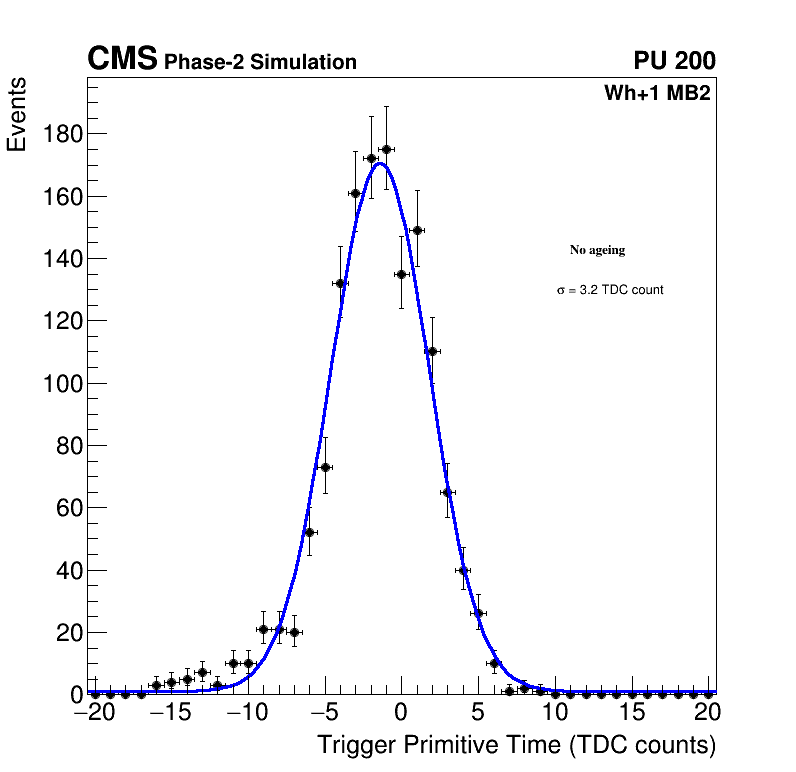
\includegraphics[width=0.45\textwidth]{Images/hTime_AMCorrelated_Wh+1_MB2_P2.pdf}
\end{center}
\caption{\textcolor{red}{DUMMYPLOTS} TP time distribution for correlated TPs in Wh+1 MB2. End of HL-LHC ageing is applied to hits before TP generation.}
\label{dts:fig:time}
\end{figure}


\subsection{Rate studies}

TP rates have been computed for the AM algorithm using the previously described simulated sample, with and without considering ageing end of HL-LHC effects. For each event, only the chambers not crossed by offline reconstructed muons were considered. Without ageing, rates for DT TPs with at least 4 hits are in fair agreement with the ones extrapolated from Phase-1 data, of the order $\sim0.5$~MHz at $10\times10^{34}~$cm${}^{-2}$s${}^{-1}$ in MB1 external wheels \cite{muontdr}. Rates elsewhere are at least a factor of two smaller, with most chambers having one order of magnitude less rate then the MB1 external wheels. Ageing reduces the trigger primitive rates as expected by the hit efficiency loss. In the MB1 external wheels, the rate is around three times smaller. All these estimated rates fit within the specification for the new Phase-2 L1 trigger system.


\section{Firmware implementation}

The AM trigger algorithm, already designed in a firmware-oriented approach, has been ported to VHDL in order to estimate the FPGA resources required. This implementation has been validated with real data using emulator-to-firmware comparisons in prototype boards.

The present firmware implementation performs the TP generation in the r-$\phi$ view of the DT chamber and its consistent with the algorithm description included in Section~ \ref{sec:dts:description}. However, some small differences are present, mainly due to practical constraints. In particular, confirmed qualities are not implemented in the firmware version for the moment. 

The present implementation of the algorithm has been performed in a \textcolor{red}{FPGA family} FPGA. On top of the AM algorithm logic, several functionalities have been included to allow the control and operation of the system.

\subsection{Firmware-Emulator comparison}

In order to study the level of agreement between the current emulator and the firmware implementation, a series of studies have been done at a test stand at CIEMAT. In these tests, the input is given by the DT hits from the previously described simulated sample, coming from all chambers in the CMS detector. These hits are stored in a file and injected at the input buffers of the \textcolor{red}{BOARDNAME} board. These hits already have the Phase-2 data format and are injected at a predefined time, emulating the behaviour of the OBDT. Hits go through all the trigger chain inside the \textcolor{red}{FPGANAME}, and TPs are generated in the board and are read out. The emulator is also run on the same sample, so results from both emulator and firmware can be compared.

The first test tries to quantify how many TPs are produced in both emulator and firmware and what is the level of additional TPs produced in each implementation. To do so, for any given primitive output by the firmware(emulator), a corresponding primitive is searched for in the emulator(firmware) output, sharing the same fitted hits with the same laterality assignments. This \textit{matching efficiency} is quantified in Table~\ref{dts:tab:fwemu}, where the percentage of matched primitive pairs is shown per TP quality. This matching is in general greater than 97\% for all qualities (except quality 6, which suffers from a high statistical uncertainty).


\begin{table}[h!]
\begin{center}
\begin{tabular}{c | c | c}
Quality & Matching w.r.t.~emulator (\%) & Matching w.r.t.~firmware (\%) \\\hline
1 & $95.11 \pm 0.24$ & $97.95 \pm 0.16$ \\
3 & $98.37 \pm 0.24$ & $99.35 \pm 0.15$ \\ 
6 & $78.95 \pm 6.5$  & $81.1 \pm 6.4$   \\
7 & $94.0 \pm 1.1$   & $94.8 \pm 1.0$   \\
8 & $100.00 ^{+0.0}_{-0.48}$ & $99.22 \pm 0.20$
\end{tabular}
\caption{Matching efficiency per quality between the firmware and the emulator implementations. The second(third) column shows the percentage of firmware(emulator) TPs that could also be found in the emulator(firmware). Note that, as the confirmation is not included in the firmware implementation, it is also skipped in the emulator version used for these tests, so no quality 2 and 4 TPs are produced.}
\label{dts:tab:fwemu}
\end{center}
\end{table}

The second test studies the agreement in the parameter values computed by both firmware and emulator. This is done by comparing the obtained parameters between pairs of emulator-firmware TPs that fit the same hits with the same laterality assignment. In Fig.~\ref{dts:fig:fwemu_time}, the left panel shows the difference between the TP BX obtained by the emulator (in blue) or the firmware (in red) and the event BX. As shown in the insert, agreement in time is at the level of least significant bit (1~TDC count). Similarly, the right panel compares the time fitted by the emulator (in blue) and the firmware (dashed red) once substracted the BX from the event (multiplied by 32 in order to convert the BX number to units of TDC counts). Perfect agreement between both curves can be seen.


\begin{figure}
\begin{center}
\subfloat{\includegraphics[width=0.45\textwidth]{Images/DeltaBXIns}}
\subfloat{\includegraphics[width=0.45\textwidth]{Images/DeltaTimeDist}}
\end{center}
\caption{\textcolor{red}{DUMMYPLOTS} Left: Difference in BX assignment between emulator TPs and event BX (blue) and firmware TPs and event BX (red). Insert shoes agreement in the fitted time value at the level of Least Significant Bit (1 ns). Right: Difference between TP time and the event BX $\cdot$ 32, as obtained by the emulator (blue) and the firmware (dashed reds). In both plots, only pairs of primitives fitting the same hits with the same laterality assignment are considered.}
\label{dts:fig:fwemu_time}
\end{figure}

In Fig.~\textcolor{red}{posición y slope}, the left panel shows a comparison between the trigger positions obtained by emulator and firmware. The right panel shows the distributions of local direction as obtained by emulator (blue) and the firmware (dashed red). In both cases, the corresponding inserts show agreement at the level of Least Significant Bit on these variables.


\section{AM performance in the CMS DT Slice Test}

During LS2, a complete exercise has been made to instrument one sector (Wheel +2, Sector 12) of the CMS detector with the new Phase-2 DT electronics prototypes. Chamber signals were split into the four DT stations, so they can be readout at the same time with the Phase-1 electronics and the new OBDT boards. In the current setup, each OBDT covers one superlayer, except in the MB4, where two OBDTs per superlayer are required. The time digitization performed by the OBDT has a time bin of \textcolor{red}{1 TDC count}, 







%\bibliographystyle{plain}
%\bibliography{../biblio.bib}

\end{document}

